\section{Flow of a Complete Vector Field}
Let $(\M, \calO, \calA)$ be a smooth manifold and $X$ be a vector field on $\M$. 
\begin{defn}[Integral Curve of a Vector Field]
    A curve $\gamma: \mathbb{R} \supseteq I \to \M$ is called an \textit{integral curve}
    of $X$ if
    \begin{equation}
        v_{\gamma, \gamma(\lambda)} = X_{\gamma(\lambda)}\,,
    \end{equation}
    \textit{i.e.}\ at every point the tangent vector of the curve is the vector of the
    vector field at that point, see figure~\ref{fig:integralCurve}.
\end{defn}
\begin{figure}[tbh]
    \centering
    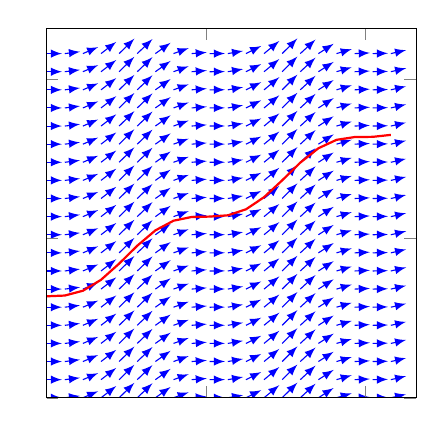
\begin{tikzpicture}
        \begin{axis}[
                width=0.6\textwidth,
                view={0}{90},
                domain=0:2*pi+0.5,
                y domain=0:2*pi+0.5,
                xmax=2*pi+1, ymax=2*pi+1,
                samples=20,
                axis equal image,
                %axis lines = center,
                xtick = {0,3.14,6.28},
                ytick = {0,3.14,6.28},
                xticklabels = {},
                yticklabels = {}
            ]
            \addplot3 [blue, quiver={u={1}, v={sin(deg(x))^2}, scale arrows=0.3, every arrow/.append style={-latex}}] {x};
            \addplot [thick, red] {2-sin(deg(x))*cos(deg(x))/2+x/2};
        \end{axis}
\end{tikzpicture}
    \caption{One integral curve of a vector field.
    Plot adapted from~\cite{texstackexchange:integralCurve}}
    \label{fig:integralCurve}
\end{figure}
\begin{note}
    Think of $X$ as the velocity of water molecules in a river and $\gamma$
    the trajectory of a paper ship that you throw into that river.
\end{note}
\begin{defn}[Complete Vector Field]
    A vector field $X$ is said to be \textit{complete} if all integral curves have
    $I=\mathbb{R}$.
\end{defn}
\begin{note}
    You cannot just reparametrize the curve with something like an arctan, because
    then it is no longer an integral curve!
\end{note}
\begin{theorem}[]
    A compactly supported smooth vector field is complete.
    (Compact: Any open cover a finite subcover, we don't have to understand this at
    the current point.)
\end{theorem}
\begin{defn}[Flow of a Vector Field]
    The \textit{flow of a vector field} $X$ is a one-parameter family
    \begin{align}
        h^X: \mathbb{R}\times\M &\to \M\,,\\
        (\lambda, p) &\mapsto \gamma_p(\lambda)\,,
    \end{align}
    where $\gamma_p:\mathbb{R}\to\M$ is the integral curve of $X$ with
    $\gamma(0) = p$.
\end{defn}
\begin{note}
    For a fixed $\lambda\in\mathbb{R}$
    \begin{equation}
        h^X_\lambda: \M \to \M, \quad\text{smooth}\,,
    \end{equation}
    it takes points of the manifold and pushes them further along the 
    curve~$\gamma$ a parameter distance $\lambda$.
    The same can be done for a set $S\in\M$ and in general
    \begin{equation}
        h^X_\lambda(S) \neq S\,,\quad(\text{if }X\neq 0)\,.
    \end{equation}
\end{note}

\subsection[Lie Subalgebras of the Lie Algabra of Vector Fields]{Lie Subalgebras of the
    Lie Algabra $(\Gamma(\T \M, [\cdot,\cdot])$ of Vector Fields}
    \paragraph{Lie algebra:}
    \begin{equation}
        \Gamma(\T\M) = \{\text{set of all vector fields}\}
    \end{equation}
    is a $C^\infty(\M)$-module.
    We can also restrict ourselfs to the $\mathbb{R}$-vector space,
    \textit{i.e.}\ only multiplication by numbers, not functions.
    Then the \textit{Lie bracket} is $[X,Y]\in\Gamma(\T\M)$, where again
    \begin{equation}
        [X,Y]f := X(Yf) - Y(Xf)\,,
    \end{equation}
    with properties
    \begin{enumerate}
        \item $[X,Y] = - [Y,X]$\,,
        \item $[\lambda X + Z, Y] = \lambda[X,Y] + [Z, Y]$\,,
        \item $[X,[Y,Z]] + [Z,[X,Y]] + [Y, [Z,X]] = 0$ (Jacobi identity).
    \end{enumerate}
    Every structure that fulfills above items and so especially
    $(\Gamma(\T\M), [\cdot,\cdot])$ is called a \textit{Lie algebra}.

    \paragraph{Lie subalgebra:}
    Let $X_1, \ldots, X_s$ be $s$ many vector fields on $\M$, such that
    \begin{equation}
        [X_i, X_j] \ C^k{}_{ij} X_k\,,\quad\forall i,j=1,\ldots,s\,,
        \label{eq:lieSubalgebra}
    \end{equation}
    with the \textit{structure constants} $C^k{}_{ij}\in\mathbb{R}$.
    Then
    \begin{defn}[Lie subalgebra]
        \begin{equation}
            (\mathrm{span}_\mathbb{R}\left\{ X_1,\ldots,X_s \right\}, [\cdot,\cdot])\,,
        \end{equation}
        with eq.~(\ref{eq:lieSubalgebra}) is called a \textit{Lie subalgebra}.
    \end{defn}
    \begin{example}[(on $S^2$)]
        \begin{align*}
            [X_1, X_2] = X_3\,,
            [X_2, X_3] = X_1\,,
            [X_3, X_1] = X_2\,,
        \end{align*}
        $(\mathrm{span}_\mathbb{R}\left\{ X_1,\ldots,X_s \right\}, [\cdot,\cdot])=so(3)$.
        Note that we did not need any metric, only a smooth manifold $(S^2, \mathcal{O}_\text{sd}, \calA)$ was needed.
        The vectors are given in a chart $(\theta, \phi)$ by
        \begin{align*}
            X_1(p) &=  -\sin\left( \phi(p) \right)\frac{\partial}{\partial \theta} -
            \cot\left( \theta(p) \right) \cos\left( \phi(p) \right)\frac{\partial}{\partial \phi}\,,\\
            X_2(p) &= \cos\left( \phi(p) \right)\frac{\partial}{\partial \theta} - 
            \cot\left( \theta(p) \sin\left( \phi(p) \right) \right)\frac{\partial}{\partial \phi}\,,\\
            X_3(p) &= \frac{\partial}{\partial \phi}\,.
        \end{align*}
    \end{example}

    \subsection{Symmetry}
    \begin{defn}[Symmetry of a Metric]
        An $s$-dimensional Lie subalgebra $(L, [\cdot,\cdot])$ is said to be a
        \textit{symmetry} of asymmetry metric tensor field $g$ if
        $\forall X\in L$ (vector field), $\forall A,B \in \T_p\M$,
        $\forall \lambda \in \mathbb{R}$:
        \begin{equation}
            g\left( (h^X_\lambda)_* (A), (h^X_\lambda)_*(B) \right) = g(A,B)\,,
        \end{equation}
        or put differently:
        \begin{equation}
            (h^X_\lambda)^* g = g\,.
        \end{equation}
    \end{defn}

    \subsection{Lie Derivative}
    If $\forall X \in L$ the \textit{Lie derivative} of the metric
    \begin{equation}
        \mathcal{L}_X g:= \lim_{\lambda \to 0}
        \frac{(h^X_\lambda)^* g - g}{\lambda} =0\,,
    \end{equation}
    then $L$ is a symmetry of $g$.

    \begin{defn}[The Lie Derivative $\mathcal{L}$]
        On a smooth manifold $(\M, \calO,\calA)$, the \textit{Lie derivative}
        $\mathcal{L}$ sends a pair of a \textit{vector field} $X$ and a
        $(p,q)$-\textit{tensor field} $T$ to a $(p,q)$-tensor field 
        $\mathcal{L}_X T$ such that
        \begin{enumerate}
            \item $\Lie_X f = X f$\,, $f\in C^\infty(\M)$\,,
            \item $\left(\Lie_X Yp\right)_p = [X,Y]_p$\,, $Y\in \Gamma(\T\M)$\,,
            \item $\Lie_X(T+S) = \Lie_X T + \Lie_X S$\,,
            \item $\Lie_X\left(T(\omega, Y)\right) = (\Lie_X T) (\omega, Y) +
                T\left( \Lie_X \omega, Y \right) + T(\omega, \Lie_X Y)$\,,
            \item $\Lie_{X+Y}T = \Lie_X T + \Lie_Y T$\,.
        \end{enumerate}
    \end{defn}

    It is a good exercise to calculate the components of the Lie derivative in a chart:
    \begin{align*}
        (&\Lie_X Y)^i = \diff x^i [XY - YX] \\
        &= \diff x^i \left[ X^m \frac{\partial}{\partial x^m}Y^n \frac{\partial}{\partial x^n}
        - Y^n\frac{\partial}{\partial x^n} X^m \frac{\partial}{\partial x^m}\right]\\
        &= \diff x^i \left[ X^m \left( \frac{\partial}{\partial x^m} Y^n \right) \frac{\partial}{\partial x^n}
        - Y^n \left( \frac{\partial}{\partial x^n} X^m \right)\frac{\partial}{\partial x^n}\right]\\
        &= X^m\frac{\partial}{\partial x^m}Y^i - Y^m \frac{\partial}{\partial x^m}X^i\,,
    \end{align*}
    where we have used the product rule for derivatives and that the second derivatives commute.
    Summary:
    \begin{align}
        \left( \Lie_X Y \right)^i &= X^m\frac{\partial}{\partial x^m}Y^i - Y^m \frac{\partial}{\partial x^m}X^i\,,\\
        \left( \nabla_X Y \right)^i &= X^m\frac{\partial}{\partial x^m}Y^i + \Gamma^i{}_{ab}X^a Y^b\,,
    \end{align}
    and in general for the Lie derivative every index up comes with a ``-'' and every index down
    comes with a ``+''.
    \begin{equation}
        \boxed{%
         \left( \Lie_X T \right)^i_j = X^m \frac{\partial}{\partial x^m}\left( T^i_j \right) -
        \frac{\partial X^i}{\partial x^m}T^m_j
        + \frac{\partial X^m}{\partial x^j}T^i_m
    }
    \end{equation}
    \begin{center}
        \fbox{\parbox{0.42\textwidth}{%
                $\nabla_X$: index up comes with $+\Gamma$, index down with $-\Gamma$.\\
                $\Lie_X$: index up comes with $-Y^s \partial/\partial x^s$, index down with +.
            }
        }
    \end{center}
    \begin{note}
        The \textit{connection} $\nabla_X$ is $C^\infty(\M)$-linear in $X$,
        whereas the \textit{Lie derivative} $\Lie_X$ is not, it is just $\mathbb{R}$-linear.
        Also we only have to give a vector $X$ to $\nabla_X$ in order to take the \textit{derivative}
        of a tensor field.
        On the other side $\Lie_X$ needs a vector field $X$.
        For $\nabla_X$ we had to introduce a new structure, the $\Gamma$s, the Lie derivative $\Lie_X$
        needs no new structure.
    \end{note}
    \begin{note}
        Use
        \begin{equation}
            0 = \left( \Lie_X g \right)_{ij} = \ldots
        \end{equation}
        to check whether a metric features a symmetry.
    \end{note}

